\documentclass{article}
\usepackage{amsmath, amssymb,amsfonts,tikz}
\usetikzlibrary{shapes,arrows,calc,positioning}
\title{Algorithms \& Complexity: Lecture 1}
\author{Sam Barrett}
\newcommand{\qs}{q_{\texttt{start}}}
\newcommand{\qh}{q_{\texttt{halt}}}

\begin{document}

\maketitle

\section{Defining the Turing machine model}
\label{sec:definition}

In order to talk about the time taken or the space used by an algorithm, we require a precise \textbf{model of computation}. There are many proposed models, we will focus on the Turing machine as defined by Arora and Barak in their book.

\subsection{Arora-Barak Turing machines}

\subsubsection{Tapes}

A Turing machine is defined as having $k$ tapes where $k \geq 2$

\begin{itemize}
  \item The first tape is the \textit{input tape} and is \textbf{read-only}
  \item The $2..k-1$ tapes are \textit{work } tapes and are \textbf{read-write}
  \item The $k^{th}$ tape is the \textit{output} tape.
\end{itemize}

Each tape has a leftmost cell and \textit{potentially} infinitely many cells to the right of it. Potentially infinite meaning that at any given time, there are a finite number of cells but we can infinitely extend the tape over time.

Each tape has a \textbf{head} that sits on a cell and can move left and right.

\subsubsection{Alphabet}

A Turing machine also has an alphabet, denoted $\Gamma $. This is a \textbf{finite} set and it's elements are called \textit{symbols}. There are 4 primary symbols: $\rhd, \Box, 0, 1 $.

Here:

\begin{itemize}
  \item $\{ 0,1 \}^{*} $ is the set of bitstrings, the empty string is denoted with $\varepsilon$.
  \item $\rhd$ is the left-of-tape symbol and $\Box$ is the blank symbol
\end{itemize}

At any point in time, each cell of each tape contains a symbol. All but a finite number will be blank ($\Box$)

\subsubsection{Inital configuration}

The input tape has $\rhd$ on the leftmost cell, then a bitstring (the \textbf{input}) and the rest of the tape is blank. The work tapes (including the output tape) have $\rhd$ on the leftmost cell and the rest are blank.
Each tape starts with it's head on it's the leftmost cell.

\subsubsection{Computation step}

In a single step of computation the machine:

\begin{itemize}
  \item reads the character at each tape head
  \item writes a character at each work tape head
  \item may move each tape head to the left or to the right. \textbf{note: our tapes are not recursive, if a head on the leftmost cell moves left, it stays put}
\end{itemize}

\subsubsection{Formal definition}

A \textbf{Turing machine} is defined as a (6) tuple, $M = (k, \Gamma, Q, q_{\texttt{start}}, q_{\texttt{halt} },\delta )$ consists of the following data:

\begin{itemize}
  \item the number of tapes, $k$, $k \geq 2$
  \item the alphabet $\{ 0,1,\rhd,\Box \} \subseteq \Gamma $
  \item a finite set of $Q$ states, including the start state $q_{\texttt{start} }$ and the halt state $q_{\texttt{halt} }$
  \item a transition function, $\delta: Q \times \Gamma^{k} \rightarrow Q \times \Gamma^{k-1}\times \{ L,R,S \}^{k} $
        Where:
        \begin{itemize}
          \item the initial $Q$ is the state at the start of transition
          \item $\Gamma^{k}$ is the set of symbols read
          \item the final $Q$ is the state at the end of transition
          \item $\Gamma^{k-1}$ is the set of symbols written
          \item $\{ L,R,S \}^{k} $ is the set of movement instructions where:
                \begin{itemize}
                  \item $L$ means \textit{move left}
                  \item $R$ means \textit{move right}
                  \item $S$ means \textit{stay}
                \end{itemize}
        \end{itemize}

        \textbf{Note: we read $k$ symbols but only write $k-1$ symbols as we do not write on the input tape, we also have $k$ movement instructions as we are able to move on all $k$ of the tapes.}
\end{itemize}

\subsubsection{Example transition}

Say we have $k=$, and $\Gamma = \{ \rhd, \Box, 0 ,1 \} $ and $Q = \{ 4,5,6,7,8 \} $ with $q_{\texttt{start} } = 4$ and $q_{\texttt{halt} } = 8$.
We are currently in state 7 and the three tapes respectively say 1 (input), 1 (work) and $\Box$ (output).

Say that $\delta(7, \langle 1,1 \Box \rangle ) = (5, \langle 0, \Box \rangle , \langle L,L,S \rangle )$ then we:

\begin{itemize}
  \item transition to state 5
  \item overwrite thje 1 on the work tape with 0
  \item overwrite the $\Box$ on the output tape with $\Box$ (no change)
  \item move left on the input tape (if possible)
  \item move left on the work tape (if possible)
        \item stay put on the output tape
\end{itemize}

\textbf{We do not transition from the halt state (regardless of $\delta$)}

\section{Computing with Turing machines}

\subsection{Computing a function}

Given a function $f : \{ 0,1 \} ^{*} \rightarrow \{ 0,1 \} ^{* }$ a Turing machine $M = (k, \Gamma, Q, q_{\texttt{start}}, q_{\texttt{halt} }, \delta)$,

\begin{enumerate}
  \item what does it mean to say that $M$ \textbf{computes} $f$?

        It means that for every bitstring $x \in \{ 0,1 \}^{*}$, if we start in state $\qs$ with the initial configuration showing $x$ (meaning $x$ appears on the input tape and and the work tapes are blank), when we run $M$, we eventually reach $\qh$ with the output tape showing $\rhd$ on the leftmost cell and then the bitstring $f(x)$ followed by all blanks.
\end{enumerate}

Our initial configuration can be shown as:

\begin{center}
  \textbf{Input tape:}
  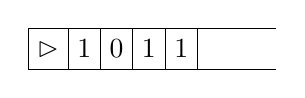
\begin{tikzpicture}[every node/.style={block},
  block/.style={minimum height=1.5em,outer sep=0pt,draw,rectangle,node distance=0pt}]


        \node (A) {$\rhd$};
        \node (B) [right = of A] {1};
        \node (C) [right = of B] {0};
        \node (D) [right = of C] {1};
        \node (E) [right = of D] {1};

        \draw (E.north east) -- ++(1cm,0) (E.south east) -- ++ (1cm,0);
               \end{tikzpicture}

\textbf{Work tapes:}
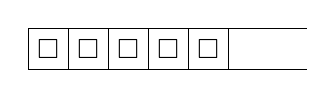
\begin{tikzpicture}[every node/.style={block},
        block/.style={minimum height=1.5em,minimum width=1em, outer sep=0pt,draw,rectangle,node distance=0pt}]

        \node (A) {$\Box$};
        \node (B) [right = of A] {$\Box$};
        \node (C) [right = of B] {$\Box$};
        \node (D) [right = of C] {$\Box$};
        \node (E) [right = of D] {$\Box$};

        \draw (E.north east) -- ++(1cm,0) (E.south east) -- ++ (1cm,0);
               \end{tikzpicture}

\textbf{Output tape: (also a work tape)}
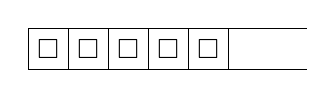
\begin{tikzpicture}[every node/.style={block},
        block/.style={minimum height=1.5em,minimum width=1em,outer sep=0pt,draw,rectangle,node distance=0pt}]

        \node (a) {$\Box$};
        \node (b) [right = of a] {$\Box$};
        \node (c) [right = of b] {$\Box$};
        \node (d) [right = of c] {$\Box$};
        \node (e) [right = of d] {$\Box$};

        \draw (e.north east) -- ++(1cm,0) (e.south east) -- ++ (1cm,0);
\end{tikzpicture}
\end{center}


Given that $f(x) = 0110111$, our required output tape will then be as follows:

\begin{center}
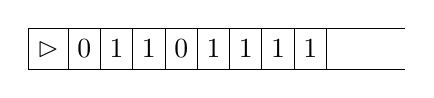
\begin{tikzpicture}[every node/.style={block},
        block/.style={minimum height=1.5em,minimum width=1em,outer sep=0pt,draw,rectangle,node distance=0pt}]

        \node (a) {$\rhd$};
        \node (b) [right = of a] {0};
        \node (c) [right = of b] {1};
        \node (d) [right = of c] {1};
        \node (e) [right = of d] {0};
        \node (f) [right = of e] {1};
        \node (g) [right = of f] {1};
        \node (h) [right = of g] {1};
        \node (i) [right = of h] {1};

        \draw (i.north east) -- ++(1cm,0) (i.south east) -- ++ (1cm,0);
\end{tikzpicture}
\end{center}

If the machine, $M$ does \textit{this} for every bitstring $x$ then we say it \textbf{computes} $f$. In the Arora-Barak definition, it does not matter what is on the work tape at the end of execution or the location of the work heads.

\end{document}
